\zlabel{firstpagetocount}       % DO NOT REMOVE! Used for counting number of pages of main text

% Part Labels Explanation:
% Labels in the form \label{chapter:<part_name>} are used to categorize chapters into specific parts of the thesis structure.
% These labels are essential for calculating the ratio of text dedicated to different thesis sections (e.g., Introduction, Methodology, Results, Discussion, Summary).
% Allowed labels:
% - chapter:introduction -> Introduction (<10% of the text).
% - chapter:method       -> Methodology (<20% of the text).
% - chapter:results      -> Results (30–40% of the text).
% - chapter:discussion   -> Analysis, Discussion, and Conclusions (30–40% of the text).
% - chapter:summary      -> Summary (<0.5 pages).
% How to use: Add a \label{chapter:<part_name>} for each chapter to indicate its part. 
% These labels ensure consistency and allow automated tests to validate the thesis structure.

\chapter{Sissejuhatus}\label{chapter:sissejuhatus} % This command creates a numbered chapter titled "Sissejuhatus" (Estonian for "Introduction"). The \label{chapter:introduction} assigns a label to the chapter, allowing you to reference it later (e.g., \ref{chapter:introduction}).
Antud magistritöö põhieesmärgiks on võrrelda masinõppe meetodeid ja tuua välja täpseim mudel, mis suudaks tuvastada metsaraiet satelliidipiltidelt. Mida aeg edasi seda rohkem on riigid hakanud mõistma kui tähtis on metsamajandus, metsade säilitamine ja hoidmine. Tehnoloogia pideva arenguga on hakatud ka otsima viise kuidas riik või kogukond saaksid paremat ülevaadet suurtest metsaga kaetud aladest. Metsa seireks kasutatakse peamiselt mehitamata õhusõidukeid (Unmanned Aerial Vechicles), maapealseid sensoreid, satelliidipildi töötlust, vabatahtlike kaasavaid rakendusi (Crowdsourcing Applications) \cite{cheungPerimeterDefense42015}.

Praegusel hetkel kasutatakse Eestis mõni aasta tagasi Keskkonnaagentuuri ja Tartu Ülikooli koostöös väljatöötatud statistika mudelit, mis raie tuvastamiseks kasutab suvasalu (Random forest) algoritmi \cite{TartuUlikooliTeadlased2020} satellidi piltidelt. Selle mudeli esmased tulemused olid paljulubavad, aga peale mõndaaegset kasutamist pole see ikkagi rahuldavaid tulemusi andnud ja mudeli kasutajad on sunnitud siiski manuaalseid viise kasutama.

Euroopa Liidu kaugseireprogrammt Copernicus võimaldab Eesti riigil koguda satelliidi pilte andmekeskusesse Esthub \cite{maa-ametRiiklikSatelliidiandmeteKeskus}. Lisaks muule infole, mida hallatakse Copernicus-es ja seeläbi ka Esthub-is, on kasutusel informatsioon mis tuleb erinevatelt Sentineli nime kandvatelt satelliitidelt \cite{InfrastructureOverviewCopernicus}. Kuna Sentinel-2 on juba 2015. aastast töös olnud, sisaldab laia valikut valgusribasid ning on tiheda korduskülastus sagedusega \cite{Sentinel2OverviewScienceDirect}, siis keskendub käesolev magistritöö peamiselt sellele sateliidi tüübile.

Sellest tulenevalt ona üheks alam eesmärgiks luua Python programm, mis hõlbustaks satelliidi piltide allalaadimist ja töötlemist. Peale andmete kogumist on plaan läbi viia tänapäevaste masinõppe mudelite võrdlus raiete tuvastamiseks. Raiet hinnatakse piksli põhise täpsusega üle pildi. Hiljuti on tehtud mitmeid uuringuid selles valdkonnas, kus kasutatakse ka suvasalu, XGBoost ja U-Net’il põhinevaid mudeli arhitektuure \cite{isaienkovDeepLearningRegular2021}, \cite{podoprigorovaRecognitionForestDamage2024}. Mõlemas uurimistöös on ka mudelite võrdlus välja toodud, aga need keskenduvad erinevatel suundadel. Esimese puhul ehitatakse mudelid kasutades rohkem pilte läbi aja, et mudel saaks paremini tuvastada muutust. Teise puhul keskendutakse erinevate lainepikkuste kombineerimisele, et tabada muutusi. 

Peale mudelite treenimist samadelt lähteandmetelt on antud magistritöös välja toodud tulemuste mõõtmine. Piksli tasemel täpsuse mõõtmiseks kasutatakse Intersection over Union - kattuvuse hinnang, Dice Coefficient - meetrika mis on põhimõtteliselt segmenteerimise F1 Score \cite{IntersectionUnionIoU}, \cite{UnderstandingDICECOEFFICIENT}. Nende tulemuste abil saab teha võrdluse erinevate tuvastusmudelite vahel, et leida neist täpseim.
 %  This command inserts the content from the file introduction.tex located in the chapters folder.

\chapter{Valdkonna ülevaade}\label{chapter:taust}
\section{Metsandus}
Metsad omavad olulist rolli nii ühiskonna igapäevaelus kui ka planeedi heaolus.
Alates mööblis kasutatavast puidust kuni paberini, millele kirjutame. Lisaks neile
nähtavatele toodetele sisaldavad paljud ravimid, kosmeetika ja pesuvahendid
metsadest saadud kõrvalsaadusi. Rohkem kui 1,6 miljardit inimest sõltub
metsadest toidu ja kütuse saamiseks ning umbes 70 miljonit, sealhulgas paljud
põlisrahvad, peavad metsi oma koduks \cite{karsentyUnderlyingCausesRapid2003}. 
Metsad varustavad meid hapnikuga, pakuvad
varjualust, töökohti, puhast vett ja toitu, olles seega inimkonna ellujäämiseks
hädavajalikud. Kuna nii paljude inimeste elu sõltub metsadest, on metsade saatus
otseselt seotud ka meie endi tulevikuga. \cite{WWFImportanceForests} 

\section{Copernicus ja EstHub}
Copernicus on üks osa Euroopa kosmoseprogrammist (EUS), mis tegeleb planeedi jälgimisega. Copernicus programmi raames, lisaks maa pealse info kogumisele, on loodud mitmeid satelliite, mis koguvad informatsiooni kosomosest. See info on kõigile kättesaadav tasuta. Selle programmiga seotud satellite kutsutakse \textbf{Sentineliks}. \cite{CopernicusCopernicus}


EstHub on Eesti riiklik satelliitandmete keskus, mis kogub ja integreerib
mitmekesiseid georuumilisi andmeid automatiseeritud protsesside kaudu.
Andmekogumine hõlmab kõrge resolutsiooniga satelliitkaadrite allalaadimist ja
standardiseerimist erinevatest allikatest. EstHubi eesmärk on koguda kokku sateliidi andmed mis katavad Eesti territooriumi. \cite{maa-ametNationalSatelliteData}

\begin{figure}[H]
    \centering
    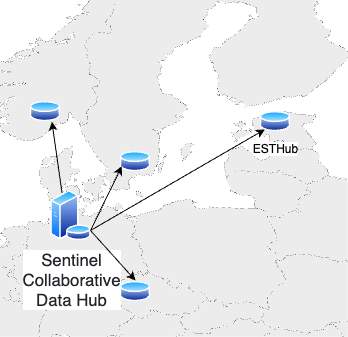
\includegraphics[width=.3\textwidth]{figures/datahubEU.drawio.png} % Includes an image from the specified path, setting the width to 50% of the text width
    \caption{Andmete liiklus EstHubi} % Provides a caption for the figure, italicizing the text
    \label{fig:esthubliiklus} % Sets a label for the figure to be referenced later
\end{figure}


\subsection{Sentinel}
Sentinel-1 on radaripõhine satelliit, mis võimaldab jälgida maapinna vajumist,
struktuuride kahjustusi ning geohazarde nagu maavärinad ja maalihked. Samuti on
see ideaalne mere- ja Arktika seireks, sealhulgas laevade jälgimiseks ning
naftareostuse tuvastamiseks. \cite{S1Applications}

Sentinel-2 missioon koosneb kahest identsest satelliidist, Sentinel-2B
(käivitatud 2017) ja Sentinel-2C (käivitatud 2024), mis töötavad koos, et
pakkuda kõrge eraldusvõimega multispektraalseid pilte Maa pindadest,
rannikualadest ja siseveekogudest iga viie päeva järel. Need andmed toetavad
rakendusi põllumajanduses, metsanduses ja maakatte klassifitseerimisel. \cite{S2Applications}

Sentinel-3 on Euroopa Maa seire satelliitmissioon, mille eesmärk on mõõta
merepinna topograafiat, mere ja maa pinnatemperatuure ning ookeani ja maa
pinnavärvi suure täpsusega. Neid andmeid kasutatakse ookeani prognoosisüsteemides,
keskkonnaseires ja kliimaseires. \cite{S3Mission}

Sentinel-5P on esimene Copernicuse missioon, mis on pühendatud atmosfääri
seirele. See kannab tipptasemel \textbf{Tropomi} instrumenti, mis kaardistab mitmeid
gaase nagu lämmastikdioksiid, osoon, formaldehüüd, vääveldioksiid, metaan,
vingugaas ja aerosoolid - kõik need mõjutavad meie hingatavat õhku, tervist ja
kliimat. \cite{S5PApplications}
\subsection{Lainepikkuste spekter}
Spektriribad on satelliitandmete analüüsimisel üliolulised, sest need
võimaldavad eristada maapinna erinevaid omadusi, lähtudes elektromagnetilise
spektri konkreetsetest lainepikkustest. Näiteks Sentinel-2 MSI instrumendi 13
spektririba hõlmavad nähtavat valgust, lähedast infrapunat ja lühilaine
infrapunat, võimaldades detailset maastiku klassifitseerimist, sealhulgas
metsade, veekogude ja muu loodusliku keskkonna eristamist. Iga ribaga seondub
kindel lainepikkuse vahemik, mida spetsiifiliste filtrite abil eraldatakse. \cite{S2Mission}
\bigskip

\begin{longtable}{llll}
    \hline
    Riba & Resolutsioon & Kasutus                          \\ 
    \hline
    B01  & 60$m \mkern3mu px^{-1}$        & Aerosool                         \\
    B02  & 10$m \mkern3mu px^{-1}$        & Sinine                           \\
    B03  & 10$m \mkern3mu px^{-1}$        & Roheline                         \\
    B04  & 10$m \mkern3mu px^{-1}$        & Punane                           \\
    B05  & 20$m \mkern3mu px^{-1}$        & Vegetatsiooni klassifitseerimine \\
    B06  & 20$m \mkern3mu px^{-1}$        & Vegetatsiooni klassifitseerimine \\
    B07  & 20$m \mkern3mu px^{-1}$        & Vegetatsiooni klassifitseerimine \\
    B08  & 10$m \mkern3mu px^{-1}$        & Lähiinfrapunariba on hea rannajoonte ja biomassisisalduse kaardistamiseks \\
    B8A  & 20$m \mkern3mu px^{-1}$        & Kitsam lähedane infrapunane  \\
    B09  & 60$m \mkern3mu px^{-1}$        & Veeaur tuvastus                       \\
    B10  & 60$m \mkern3mu px^{-1}$        & Pilvede tuvastus                      \\
    B11  & 20$m \mkern3mu px^{-1}$        & Lühilaine infrapunane 1      \\
    B12  & 20$m \mkern3mu px^{-1}$        & Lühilaine infrapunane 2      \\
         &              &                    &                              \\ \hline
    \caption{Sentinel-2 MSI spektriribad ja nende kasutusvaldkonnad}
    \label{tab:s2bands}
\end{longtable}

\subsection{Koordinaatsüsteemid ja CRS}
Koordinaatsüsteem on meetod, mille abil määratletakse ja kirjeldatakse punktide
asukohti maastikul, kasutades koordinaate. Selles kontekstis eristatakse kahte
tüüpi: geograafilised koordinaatsüsteemid, mis kasutavad laiuse ja pikkuse
väärtusi, ning projekteeritud koordinaatsüsteemid, mis teisendavad
geograafilised koordinaadid lameda kaardi koordinaatideks, kasutades
matemaatilisi projektsioone. CRS ehk koordinaatide viite süsteem määratleb
reeglid ja parameetrid, mille alusel need koordinaadid seonduvad reaalse
maastikuga. \cite{8CoordinateReference}

\section{Masinõppe meetodite kasutus kaugseires}
smt smt smt smt smt


\chapter{Lahendus}\label{chapter:lahendus}
\section{Töövahendid}


\textbf{Python}

Python on üldotstarbeline programmeerimiskeel, mida kasutatakse
laialdaselt andmeteaduse, masinõppe ja ruumiandmete analüüsi ülesanneteks
oma lihtsuse ja mitmekülgsuse tõttu. Käesolevs töös kasutatakse Pythonit
andmete töötlemiseks, mudelite treenimiseks ja tulemuste analüüsimiseks.



\textbf{Jupyter Notebookid}\nopagebreak[4]

Jupyter Notebookid pakuvad interaktiivset keskkonda, kus
saab koodi kirjutada, käivitada ja dokumenteerida ühes kohas. Need võimaldavad
dünaamilist andmeanalüüsi ja tulemuste visuaalset esitlust, muutes
uurimisprotsessi läbipaistvaks ja korduvaks. Käesolevas töös kasutatakse
Jupyter Notebooke peamiselt katsetuste tegemiseks ja tulemuste
visualiseerimiseks.



\textbf{Pandas}\nopagebreak[4]

Pandas on andmetöötluse teek, mis pakub paindlikke ja
efektiivseid andmestruktuure tabelipõhise andmetöötluse jaoks. See lihtsustab
andmete puhastamist, analüüsi ja manipuleerimist. Käesolevas töös
kasutatakse Pandast andmete lugemiseks, töötlemiseks ja analüüsimiseks.


\textbf{GeoPandas}\nopagebreak[4]

GeoPandas laiendab Pandase võimalusi, lisades tuge georuumilistele
andmetele. See võimaldab lugeda, analüüsida ja visualiseerida
ruumiandmeid ning teostada geomeetrilisi operatsioone nagu lõikumine ja
ühendamine.


\textbf{Rasterio}\nopagebreak[4]

Rasterio on Pythoni teek, mis keskendub rasterandmete lugemisele
ja töötlemisele tuginedes GDAL-ile. See võimaldab ruumiandmete analüüsi
ning laseb rasterfailidega töötada efektiivselt ja intuitiivselt. Käesolevas töös oli Rasterio peamiseks tööriist rasterandmete lugemiseks ja töötlemiseks, sealhulgas satelliidipiltide koostamiseks ja maskide genereerimiseks.

\textbf{QGIS}\nopagebreak[4]

QGIS on tasuta ja avatud lähtekoodiga töölaua GIS-tarkvara, mis võimaldab
kasutajatel andmeid visuaalselt analüüsida, redigeerida ja kaardistada. See
toetab mitmeid andmeformaate ja pakub laialdasi geoprotsessimise võimalusi,
olles populaarne nii akadeemilises kui ka professionaalses keskkonnas. Käesolevas
töös kasutatakse QGIS-i peamiselt andmete visualiseerimiseks ja
analüüsimiseks, et mõista ruumiandmete struktuuri ja omadusi.


\textbf{PostGIS}\nopagebreak[4]

PostGIS on PostgreSQL andmebaasi laiendus, mis lisab ruumiandmete töötlemise funktsionaalsuse. See võimaldab keerukaid ruumi operatsioone
ja on oluline tööriist suurte ruumiandmete kogude haldamisel ning
analüüsil. Käesolevas töös autor ise PostGIS-i ei kasutanud, kuid Keskkonnaagentuuri andmebaas, kust andmed saadi, on PostGIS-i baasil üles ehitatud. Seega on PostGIS selles uurimistöös oluline komponent andmete haldamisel ja töötlemisel.

\textbf{Riistvara}\nopagebreak[4]

Uurimistöö läbiviimisel kasutati ülikooli AI-labori ressursse. Labor koosneb ühest pea-sõlmest, mis haldab teisi masinaid, ning alamsõlmedest, mis teostavad töid. Autor kasutas ai-lab-07 sõlme CPU-intensiivsete ülesannete, nagu andmekogumi koostamine, piltide töötlemine ja kompressioon, ning konvolutsiooniliste närvivõrkude mudelite treenimiseks nagu ResNet34, ResNet50 ning MobileNetV2. Samas süvaõppe eksperimentide teostamiseks kasutati ai-lab-04 ja ai-lab-03 sõlmi, mille GPU ja mälumaht võimaldasid keerukamate mudelite treenimist. Selline ressursside jaotus aitas töövoogu optimeerida ja tagada tööde sujuva teostuse vastavalt konkreetsetele arvutusvajadustele. Ülevaate kasutatud ressurssidest leiab Tabelist \ref{tab:hardwareused}.

\begin{table}[H]
\caption{Kasutatud riistvara}
\label{tab:hardwareused}	
\begin{longtable}{lllll}
    \hline
    Sõlm & Protsessor & Mälu & GPU & GPU mälu                         \\ 
    \hline
    ai-lab-03 & 7975WX 32-cores/64-threads & 384 GB & NVidia RTX6000Ada & 48 GB    \\
    ai-lab-04 & 3970X 32-cores/64-threads & 128 GB & NVidia 4090 & 24 GB      \\
    ai-lab-07 & 3060X 24-cores/48-threads & 128 GB & AMD RX6900XT & 16 GB    \\
%    &              &                    &                              \\
\hline
\end{longtable}
\end{table}
\addtocounter{table}{-1}
\section{Andmestiku loomine}
Selles peatükis käsitletakse andmestiku loomise protsessi, sealhulgas andmete kogumist, töötlemist ja maskimist. Andmestiku loomine on oluline samm igasuguste andmete analüüsimisel ja seda ka masinõppe projektide puhul. Andmete kvaliteet ja sobivus mõjutavad otseselt mudeli täpsust ja usaldusväärsust. Nagu muudes valdkondades kehtib ka informaatikas Pareto printsiip, mille kohaselt 80\% probleemidest tuleneb 20\% põhjustest. Seega on andmestiku loomine ja töötlemine äärmiselt oluline etapp, mis võib määrata kogu projekti edasise käigu.

\subsection{Raie piirkonna andmete kogumine}
Metsateatis on dokument, mille kaudu metsaomanik esitab Keskkonnaametile
kavandatavate raietööde või oluliste metsakahjustuste kohta teabe. Keskkonnaamet
kontrollib esitatud teatiste nõuetekohasust ning veendub, et kavandatav raie
vastab kehtivatele õigusaktidele. Metsateatised menetletakse ja säilitatakse
riiklikus metsaregistris. Peale edukat menetlemist võib raietöödega alustada 10 päeva peale otsust ja kuni 24 kuu jooksul. \cite{MetsateatisJaMetsaregister} Metsateatised on avalikud ja neid saab vaadata riiklikus metsaregistris.

Metsade inventeerimise ja registrisse kandmise protsess algab metsaeraldiste
täpse kaardistamisega, kasutades L‑EST97 ristkoordinaatide süsteemi, Eesti
põhikaarti, katastriüksuse plaane ning vajadusel kaugseire andmeid eraldiste
piiritlemiseks ja võimalike situatsioonielementide täpsustamiseks. Kaardistamise
tulemusena koostatakse geoinfosüsteemi metsaeraldiste kiht, kus iga eraldis on
nummerdatud ning selle pindala, arvutatuna piiripunktide koordinaatide alusel, 
esitatakse hektarites vähemalt kümnendkohani ning täpsusega 10 meetrit --- see
loob aluse usaldusväärsele pindalaarvestusele ja edaspidistele
takseerimistoimingutele. \cite{MetsaKorraldamiseJuhend}

Koostöös Keskkonnaametiga (Envir) saadi andmed metsateatistest, mis sisaldavad teavet nii metsateatise esitamise kuupäeva, metsateatise menetlemise kuupäeva, metsateatise kehtivuse alguskuupäeva kui ka metsateatise kehtivuse lõppkuupäeva kohta. Kuna riigimetsade teatised on täpsemas seisukorras, siis võeti need raieteatised selle uurimustöö aluseks. Seoses sellega et ühe lõigu peal võib olla väga väike kogus metsa, sai teatiste pärimine ümber ehitatud sedasi, et ühe metsa raie ümber kogutakse peale raie toimumist kokku ka kõik teiste raiete raadiuses asuvad piirkonnad, millel on teada kas on mets või raieala. Piirkonniti pärimine sai teostatud kasutades PostGISi liidest Postgresi andmebaasiga. Iga raie sisaldab ka endas geomeetria veergu, mis esitab polügooni kujul selle asukohta.

% TODO: eelnevas lõigus teha arusaadavamaks, mis on lõik millest räägitakse, eelnevalt juttu kuupäevadest jm teabest ja siis võib jääda segaseks. lisaks palun täpsustada: kogutakse kokku ka teised ... raadiuses asuvad piirkonnad

\begin{figure}[hb]
    \centering
    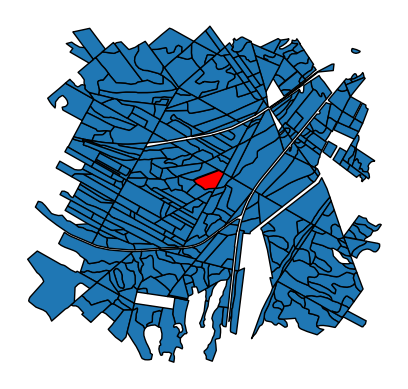
\includegraphics[width=.5\textwidth]{figures/andmestik/er_id_is10124223.png}
    \caption{Näidis ühe lageraie päringust saadud ümbrus}
    \label{fig:umbrusexample}
\end{figure}

Polügoon on geomeetriline kujund, mis määratleb kindla ala, ühendades üksteisega
punktid, et moodustada suletud piirjoon. Andmetöötluse ja ruumiandmete analüüsi
kontekstis kasutatakse polügoone, et täpselt määratleda geograafilisi alasid. \cite{WhatLocationPolygon}



\begin{figure}[H]
    \centering
    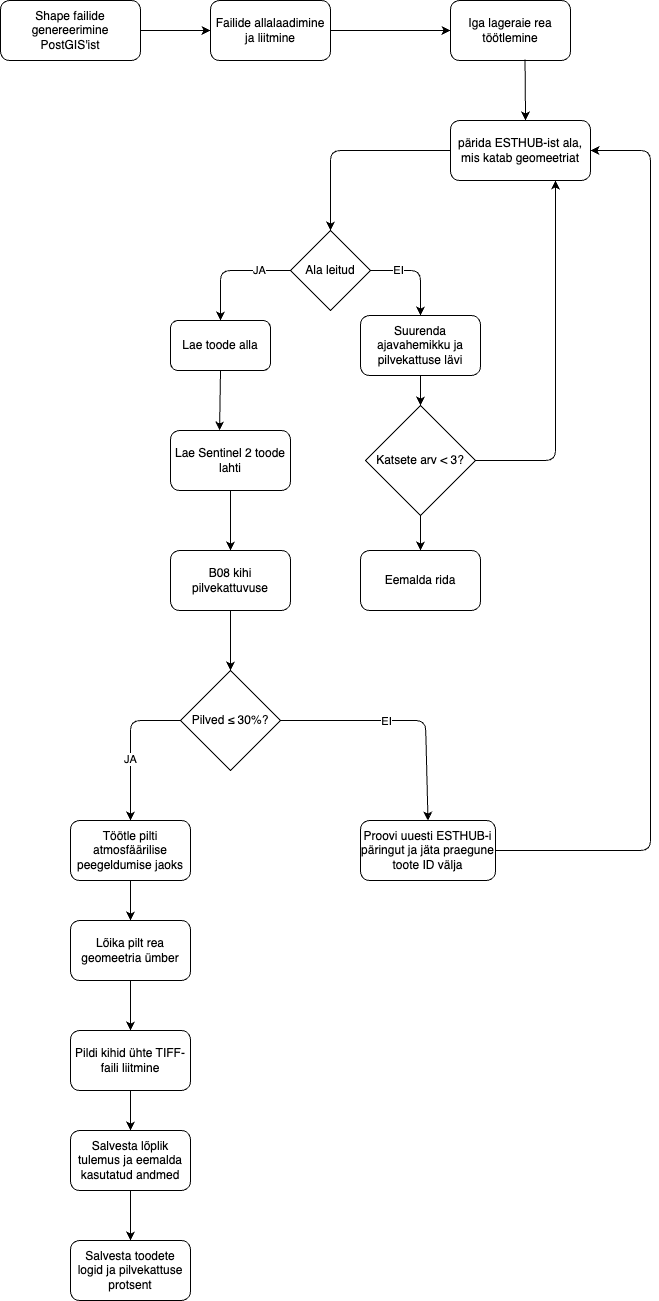
\includegraphics[width=.8\textwidth]{figures/andmestik/andmete_voog.drawio.png}
    \caption{Andmestiku loomise töövoog}
    \label{fig:terveflow}
\end{figure}


\section{Alusmudeli ülevaade}
Alusmudelid (\textit{Foundation models}) on suuremahulistel andmekogudel
ennastjuhendavalt treenitud sügavad närvivõrgud, mis toimivad üldotstarbelise
baasina mitmesuguste masinõppe ülesannete lahendamiseks. Erinevalt
traditsioonilistest mudelitest, mis on välja töötatud konkreetse ülesande jaoks
ja nõuavad eraldi treeningut, on alusmudelid eelnevalt ettevalmistatud laia
valiku ülesannete sooritamiseks --- alates loomulikust keele töötlemisest ja
tekstigeneratsioonist kuni pildiklassifitseerimise ja vastuste genereerimiseni
--- ilma täiendava märgendatud õppematerjalita. Nende mudelite
kohanemisvõime tuleneb nii suurest parameetrite hulgast kui ka enesekontrollil
põhinevast õppestrateegiast, mis võimaldab neid hõlpsasti peenhäälestada
konkreetsete rakenduste jaoks. Võimalus keskenduda mudeli peenhäälestusele ja mitte nullist treenimisele vähendab omakorda oluliselt arendusaega ja arvutiressursside vajadust.
\cite{WhatAreFoundation}

\subsection{DINO v2 ja selle kasutus}
\input{chapters/dinov2_alusmudel_võrdlus.tex}


\subsection{SAM v2  ja selle kasutus}
\input{chapters/samv2_alusmudel_võrdlus.tex}

\section{Seoste leidmine}
Selleks et tõestada antud magistritöö eesmärki segmenteerida lageraie ja metsa alasi suurte visioonimudelitega, klusterdatakse DinoV2 väljundid, et leida, kas need alad on eristatavad. Selleks on vajalik eksperdiga valideerida ühe lageraie piirkonna alad, et kindel olla, et need vastavad tõele satelliidipildilt.

Joonisel \ref{fig:näidisSadeliidiPilt} on näidispilt eksperimendist, mille käigus püüti välja selgitada, kas mudelid suudavad eristada lageraie ja metsa alasid satelliidipiltidelt. Antud Sentinel-2 andmebaasist saadud pilt sai valitud esiteks sellepärast, et see on hea nähtavusega, võimalikult vähe pilvine ja soojemal hooajal, kui pole lund ja puud on lehteis. Teiseks on käesolev pilt heaks aluseks, sest sellel on sattunud raie- ja metsapiirkondi kõrvuti, mis võimaldab erinevatesse klassidesse kuuluvate alade üleminekukohti analüüsida.

\begin{figure}[H]
    \centering
    \includegraphics[width=.7\textwidth]{figures/seose_leidmine/näidisSadeliidiPilt.png}
    \caption{Näidis sateliidi pilt}
    \label{fig:näidisSadeliidiPilt}
\end{figure}

Joonisel \ref{fig:raieInfoMask} on näha lageraie piirkond, mis on toodud välja tumedama roosana, ja metsa piirkond, mis on joonisel heleroosana. Tegemist on aladega, mis on teada Keskkonnaametile ja mille kohta on olemas ka metsateatis. Satelliidipilt on saadud Sentinel-2 andmebaasist ja sellel on kümnemeetrine resolutsioon. Antud pilt on saadud raie teostamise ajast kuni 40 päeva hiljem, seega mahub õigesse ajaraamistikku, et piisavalt täpselt hinnata metsade seisukorda.

\begin{figure}[H]
    \centering
    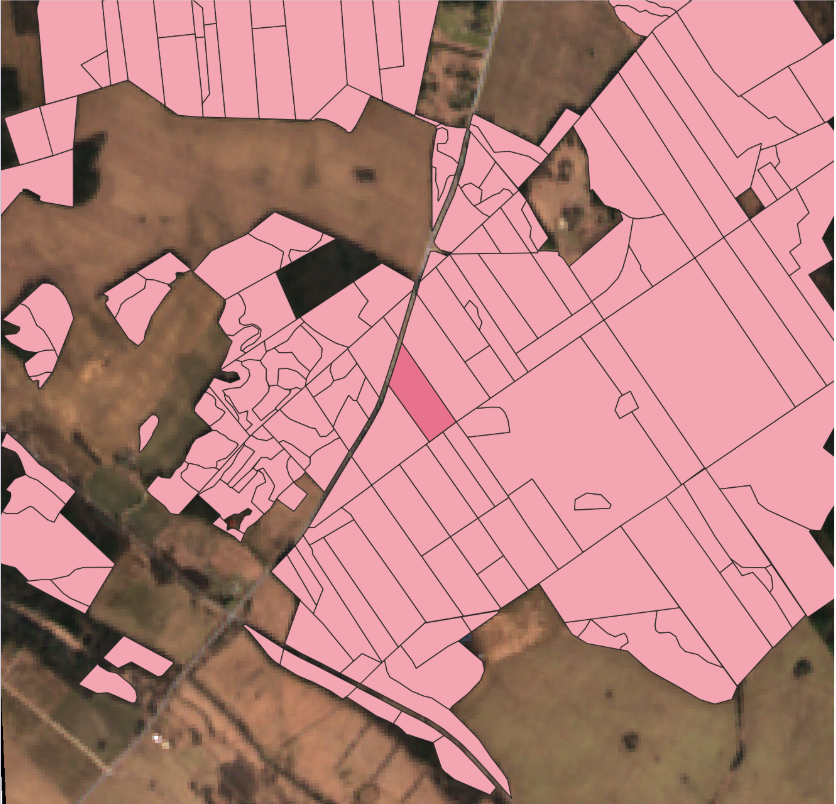
\includegraphics[width=.7\textwidth]{figures/seose_leidmine/raieInfoMask.png}
    \caption{Raie piirkonna mask sateliidi pildil}
    \label{fig:raieInfoMask}
\end{figure}

Joonisel \ref{fig:raieInfoMask_ekspert} on näha lageraie piirkond, mis on toodud välja tumepunasena ja metsa piirkond, mis on märgitud rohelisega. Ekspert on võtnud metsateatistest saadud info alade tuvastamisel aluseks, aga sellele lisaks kasutas ta ka muud teavet nagu ortofotosid ja erinevate lainepikkuste pilte, et leida täpsemad piirded metsade ja raiealade vahel. Ekspert on leidnud, et antud piirkonnas leidub alasid, mis ei vasta metsateatistes märgendatud infole. Näiteks on pildil alasid, mis teatistes on märgitud metsaks, aga silmaga vaadates kujutab hoopis raiet ja ka vastupidi. Seega on eksperdi poolt loodud mask palju täpsem ja seetõttu oli eksperdi kaasamine vajalik andmestiku loomise protsessis.

\begin{figure}[H]
    \centering
    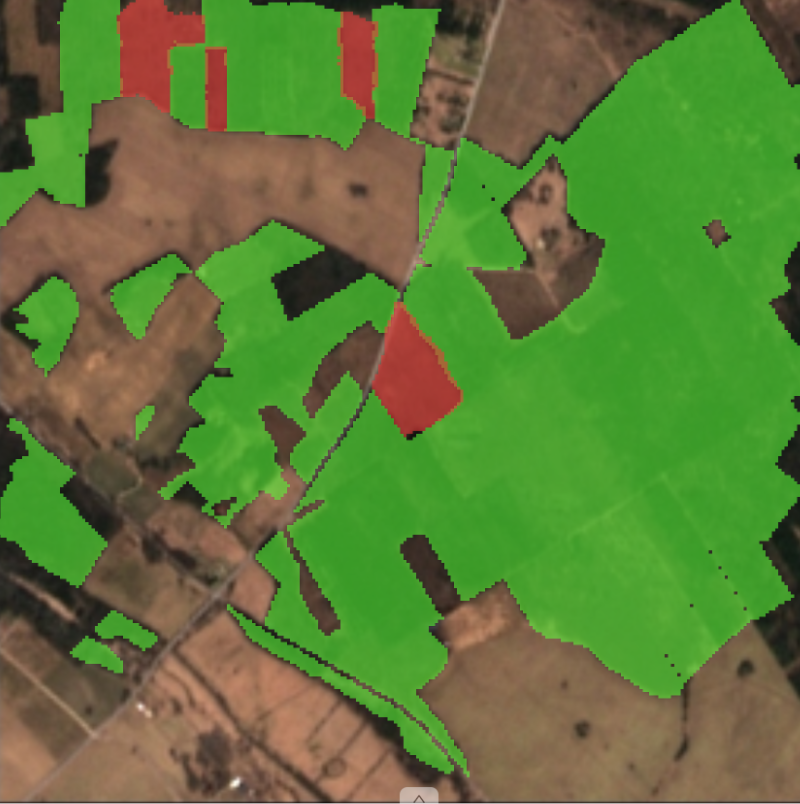
\includegraphics[width=.7\textwidth]{figures/seose_leidmine/raieInfoMask_ekspert.png}
    \caption{Raie piirkonna mask eksperdi poolt korrigeeritud}
    \label{fig:raieInfoMask_ekspert}
\end{figure}

Järgneval joonisel \ref{fig:segmenteeritudPealiskiht}, rakendati klastrianalüüsi süvaõppemudelist saadud
kõrgdimensionaalsetele tunnusevektoritele, mis esindavad sisendpildi
diskreetseid paiku. Eelkõige kasutati k-keskmise algoritmi, et grupeerida need
tunnusevektorid sarnaste semantiliste omaduste alusel. Igale pildilaigule vastav
tunnusevektor määrati ühte eelnevalt defineeritud arvu klastritesse, mille
tulemusena saadi diskreetne klastermärgis iga pildipaiga jaoks. Seejärel
visualiseeriti saadud klastermärgis pildil värvilise maskina, kus iga klaster on
esitatud unikaalse värviga, võimaldades seeläbi kvalitatiivselt hinnata mudeli
õpitud representatsioonide kohalikku sarnasust sisendpildil.

\begin{figure}[H]
    \centering
    \includegraphics[width=.7\textwidth]{figures/seose_leidmine/segmenteeritudNäidis.png}
    \caption{Segmenteeritud näidis sateliidi pildist}
    \label{fig:segmenteeritudPealiskiht}
\end{figure}

Joonisel \ref{fig:tsneDinoPatchEmbedings} on rakendatud klassipõhist klasterdamise meetodit, mille eesmärk on luua
pildimaterjalist semantiliselt sidusaid piirkondi, grupeerides pildi elemendid
eelnevalt defineeritud klassifikatsioonikategooriate alusel. Lähtudes mudeli
genereeritud klassifikatsiooniväljunditest, määratakse iga pildielement kõige
tõenäolisemasse klassi, mille alusel moodustatakse klastrid. Selle meetodi
rakendamise tulemusena saadakse segmentatsioon, kus ühte klastrisse kuuluvad
pildi osad on mudeli poolt klassifitseeritud sarnaselt. Lõppeesmärk on seeläbi
genereerida pildist arusaadavam representatsioon, mis
võimaldab interpreteerida pildi sisu semantilisel tasemel, tuues
esile objektide ja piirkondade klassipõhised seosed. Pildil on väljatoodud klass 1 mis on mets ja klass 2 mis on lageraie, lisaks sai eemaldatud tausta klass, et oleks kergem jälgida uuritavaid klasse.

\begin{figure}[H]
    \centering
    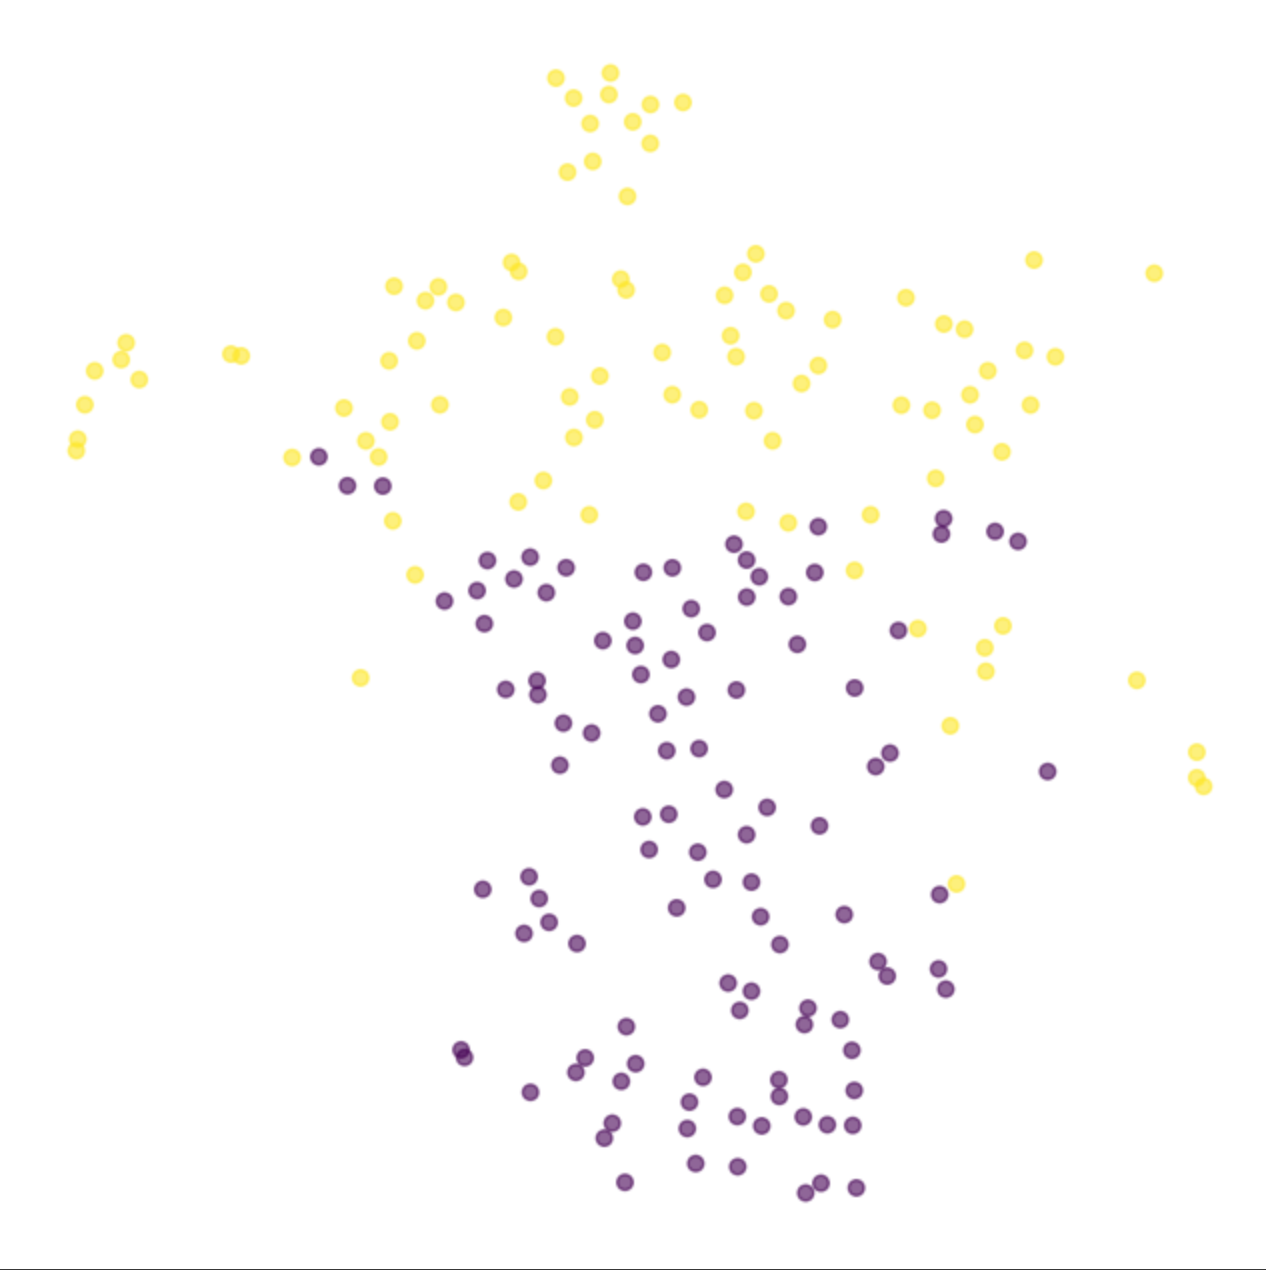
\includegraphics[width=.7\textwidth]{figures/seose_leidmine/tsneDinoPatchEmbedings.png}
    \caption{T-SNE kluster analüüs DinoV2 mudeli väljunditest}
    \caption*{klass 1 - mets, klass 2 - lageraie}
    \label{fig:tsneDinoPatchEmbedings}
\end{figure}

Siit võis näha, et lageraie ja mets on eristatavad ja annavad alust edasi uurida, millised alusmudelid suudavad paremini eristada lageraie ja metsa alasid.


\section{Treenimis protsetuurid}
\input{chapters/lähtepunkt.tex}
\input{chapters/katsed metsa ja lageraielõikude tuvastamiseks.tex}


\chapter{Tulemuste analüüs}\label{chapter:analüüs}
Selles peatükis analüüsime eelmises peatükis kirjeldatud katsete tulemusi, et mõista, kuidas erinevad mudelikonfiguratsioonid ja treeningstrateegiad mõjutavad metsastunud ja lageraielõikude tuvastamise täpsust satelliitpiltidelt. Arutatakse ka tulemuste statistilist olulisust ning võrreldakse erinevate lähenemiste efektiivsust.
\section{Tulemuste võrdlus}
\textbf{Baasjoon}

Eksperimendi käigus testiti süstemaatiliselt erinevaid hüperparameetreid, et leida optimaalne konfiguratsioon antud ülesande jaoks. 
Esitatud tulemuste analüüs näitas, et parimad mudelid
saavutasid märkimisväärselt kõrgeid Dice'i skoore, ulatudes kuni \textasciitilde
0.984. See on eriti üllatav, arvestades andmestiku koostamise väikest valimit.

Parimaks osutunud mudeli konfiguratsioon oli järgmine:
\begin{itemize}
  \item \textbf{Arhitektuur:} Unet
  \item \textbf{Enkooder:} ResNet50
  \item \textbf{Enkooderi kaalud:} ImageNet (eelkoolitatud)
  \item \textbf{Optimeerija:} AdamW
  \item \textbf{Õpisamm:} \textasciitilde 1.09e-4
\end{itemize}

Ka teised kombinatsioonid,
näiteks DeepLabV3 koos ResNet50-ga, saavutasid kõrgeid tulemusi (Dice > 0.97).
Osaliselt on tipptulemused visualiseeritud ka lisatud joonisel \ref{fig:segmentation_results}.

\textbf{Kõrgete skooride põhjused}
Kõrgeid tulemusi väikesel andmestikul võib seletada mitme teguriga.
Siirdeõpe (\textit{Transfer Learning}): ImageNet andmestikul eelkoolitatud enkooderite
kasutamine on tõenäoliselt peamine edu võti. Eelnevalt treenitud mudelid omavad
juba võimekust tuvastada üldiseid visuaalseid mustreid (nt servad, tekstuurid),
mida saab efektiivselt kohandada spetsiifilisele metsanduse segmenteerimise
ülesandele. See vähendab oluliselt vajamineva treeningandmestiku mahtu. Peaaegu
kõik parimad tulemused saavutati just imagenet kaaludega. 
Kuigi valideerimistulemused on kõrged, on väikse andmestiku kasutamine riskantne, sest alati peab arvestama ülesobitamise(\textit{overfitting}) ohuga. Samas näitab analüüs, et paljudel juhtudel valideerimis- ja treeningkahju
(val\_loss, train\_loss) vähenesid sünkroonis, mis viitab sellele, et mudelid
suutsid siiski valideerimisandmetele edukalt üldistuda ega õppinud
treeningandmeid lihtsalt pähe.

\begin{figure}[H]
    \centering
    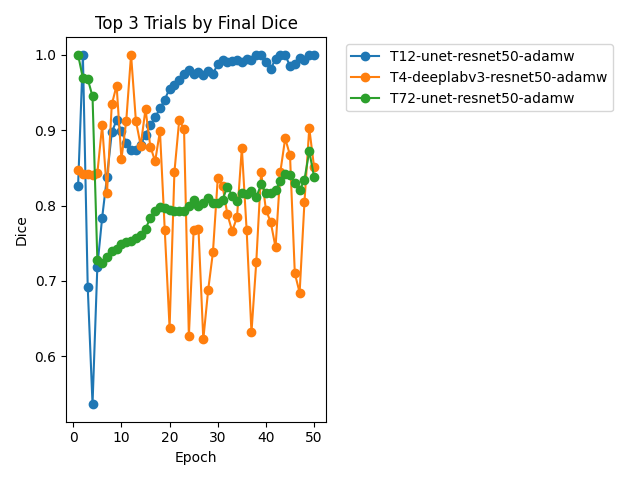
\includegraphics[width=0.8\textwidth]{figures/top3_dice.png}
    \caption{Parimad DICE tulemused erinevate mudelite vahel.}
    \label{fig:segmentation_results}
\end{figure}

Samas individuaalsed klassi tulemused (nt metsastumine vs lageraie) Dice skoorid näitasid suuresti, et mudel ei suuda
täpselt eristada metsastumist ja lageraielõike. Kõrge skoor tuleneb suuresti tagatausta suurest osakaalust pildil. Joonisel \ref{fig:sidebyside_forest_bg} on näha et ülejäänud tausta keskmine Dice skoor on 0.98, mis on väga kõrge. Aga klassipõhised tulemused näitavad, et metsastumise ja lageraielõike eristamine on keeruline. Mudelite katsed ka näitavada, et ka parimate mudelite puhul ei saa nad metsastumist ja lageraielõike eristada.

\begin{figure}[H] % Placement specifier: h-here, t-top, b-bottom
    \centering
    \begin{subfigure}[b]{0.8\textwidth} % Set width for side-by-side arrangement
        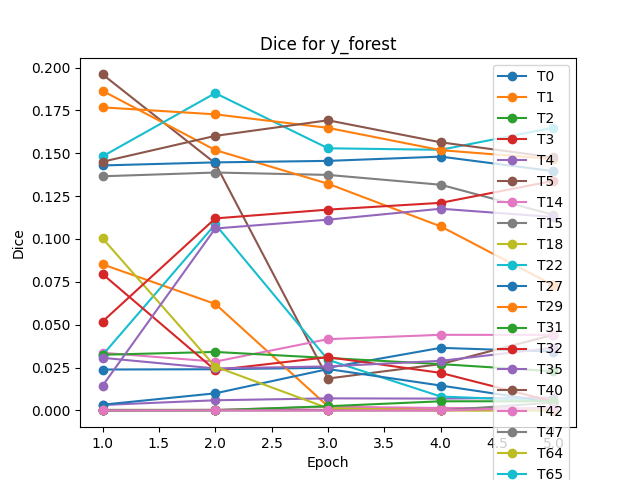
\includegraphics[width=\textwidth]{figures/tulemused/dice_per_class_y_forest.png} % Image path and full width in subfigure
        \caption{} % Leave caption empty to automatically label this subfigure as (a)
        \label{fig:dice_per_class_y_forest}
    \end{subfigure}
    % Second subfigure
    \begin{subfigure}[b]{0.8\textwidth} % Set width for side-by-side arrangement
        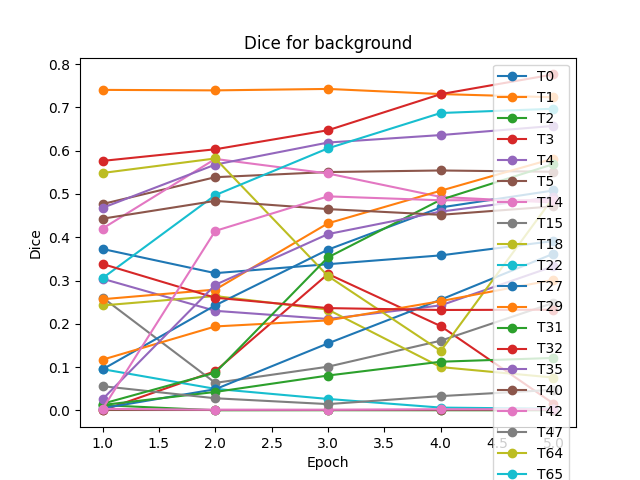
\includegraphics[width=\textwidth]{figures/tulemused/dice_per_class_background.png} % Path and full width in subfigure
        \caption{} % Leave caption empty to automatically label this subfigure as (b)
        \label{fig:dice_per_class_background}
    \end{subfigure}
    
    \caption{Tagatausta ja noore metsa segmentatsiooni Dice tulemused üle katsete} % Main caption for the whole figure environment
    \label{fig:sidebyside_forest_bg} 
\end{figure}




\textbf{Dinov2 eksperimendid}

Käesolevas uurimuses viidi läbi eksperimente, mille eesmärk oli hinnata DINOv2
raamistikul põhinevate masinõppemudelite efektiivsust satelliidipiltide
segmenteerimisel metsanduslikus kontekstis. Katsetati erinevaid Vision
Transformer (ViT) arhitektuure (nt ViT-B/14, ViT-G/14, ViT-L/14, ViT-S/14) koos
erinevate segmenteerimispeadega (nt LinearHead, SimpleHead, FPNHead,
UPerNetHead). Mudelite jõudlust hinnati keskmise Dice'i koefitsiendi, keskmise
IoU (Intersection over Union) ja keskmise täpsuse (Mean Accuracy) alusel,
jälgides neid mõõdikuid kuni 800 epohhi vältel. Treeningutingimustes varieeriti
hüperparameetreid, nagu õppimismäär (nt 1e-5, 5e-5, 1e-4), partii suurus (1, 2,
4) ning rakendati nii külmutamist (Freeze) kui ka peenhäälestamist (FineTune).
\bigskip
\begin{longtable}{llll}
    \textbf{Konfiguratsioon} & \textbf{Mean Dice} & \textbf{Mean IoU} & \textbf{Mean Täpsus} \\
    \hline
    ViTB14 LinearHead LR5e-5 BS2 E5 Freeze & 0.18 & 0.16 & 0.26 \\
    ViTB14 SimpleHead LR1e-5 BS4 E5 FineTune & 0.200 & 0.26 & 0.35 \\
    ViTG14 FPNHead LR1e-5 BS4 E5 FineTune & 0.258 & 0.28 & 0.33 \\
    ViTG14 SimpleHead LR1e-4 BS4 E5 Freeze & 0.22 & 0.275 & 0.350 \\
    ViTL14 UPerNetHead LR1e-5 BS1 E3 Freeze & 0.160 & 0.270 & 0.34 \\
    ViTS14 FPNHead LR1e-5 BS4 E5 FineTune & 0.23 & 0.25 & 0.38 \\
    \hline
    \caption{DINOv2 eksperimendi tulemused}
    \label{tab:dinov2_results}
\end{longtable}
\bigskip

Eksperimentide tulemused näitavad, et DINOv2-põhiste mudelite jõudlus satelliidipiltide segmenteerimisel sõltub oluliselt tuumvõrgu suurusest, segmenteerimispea keerukusest ja treeningustrateegiast. Suuremad tuumvõrgud (nt ViTG14) ja mitme skaala tunnuseid töötlevad pead (nt FPNHead) andsid parimaid tulemusi, saavutades keskmise IoU kuni 0,28 ja täpsuse kuni 0,38. Peenhäälestamine parandas jõudlust võrreldes külmutatud mudelitega, kuid pikaajalistes treeningutes (500–800 epohhi) ilmnes ebastabiilsus, mis viitab ületreenimisele või ebapiisavale regulatsioonile.

Soovitused edasiseks uurimistööks hõlmavad varajase peatamise ja õppimismäära ajakava rakendamist stabiilsuse suurendamiseks, samuti täiendavate arhitektuuride (nt hübriidmudelite) testimist jõudluse lae ületamiseks. Praegused tulemused pakuvad väärtuslikku alust metsanduslike satelliidipiltide segmenteerimise optimeerimiseks.


\section{Edasiarendus ja täiustamine}
\input{chapters/edasiarendus_ja_täiustamine.tex}


\chapter{Kokkuvõte}\label{chapter:kokkuvõte} 
\input{chapters/kokkuvõte.tex}

\zlabel{lastpagetocount}        % DO NOT REMOVE! Used for counting number of pages of main text
